\documentclass[11pt,letterpaper]{article}
\usepackage[lmargin=1in,rmargin=1in,tmargin=1in,bmargin=1in]{geometry}
\usepackage{../style/homework}
\usepackage{../style/commands}
\setbool{quotetype}{false} % True: Side; False: Under
\setbool{hideans}{false} % Student: True; Instructor: False

% -------------------
% Content
% -------------------
\begin{document}

\homework{15: Due 12/08}{Nothing goes over my head. My reflexes are too fast. I would catch it.}{Drax, Guardians of the Galaxy}

% Problem 1
\problem{10} Find and plot the solution to the system of equations given in the graph below:
	\[
	\fbox{
	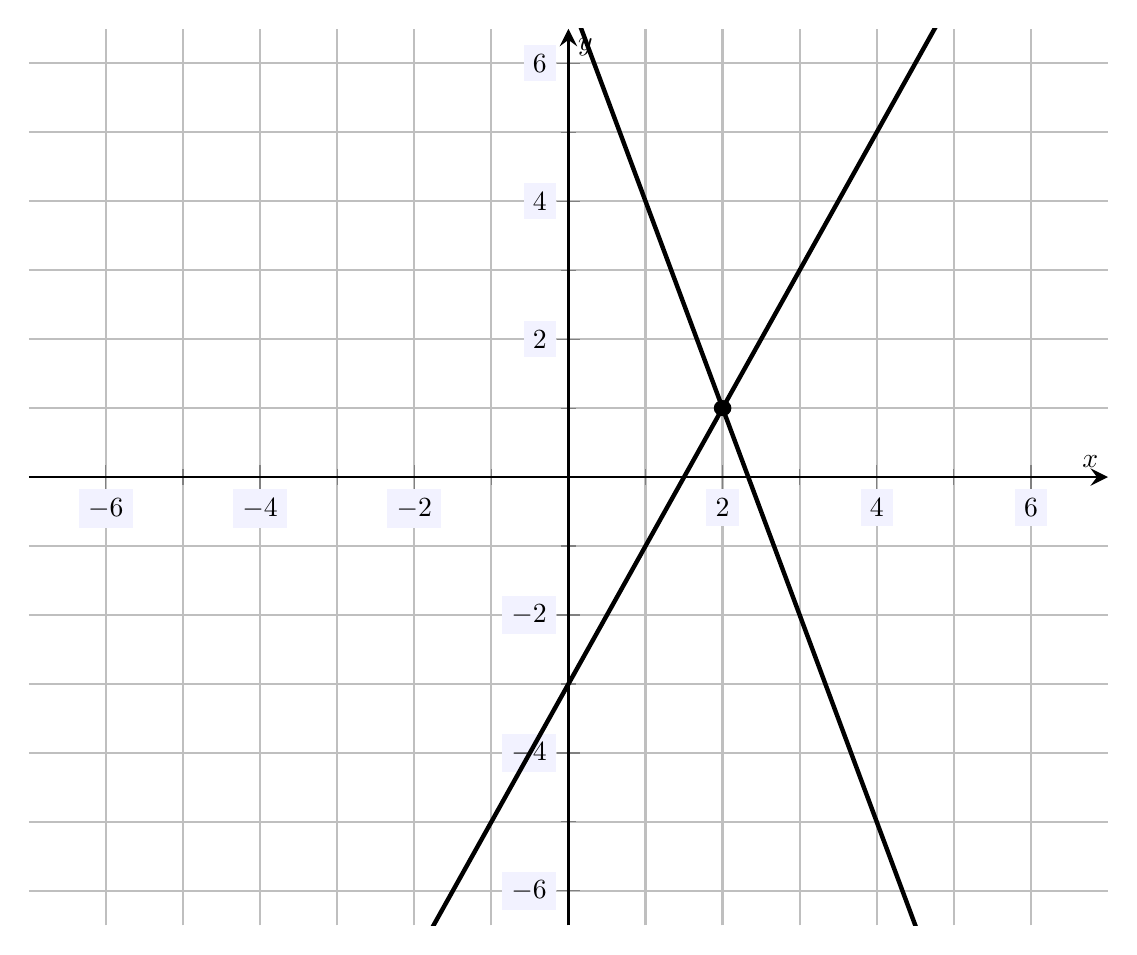
\begin{tikzpicture}[scale=2,every node/.style={scale=0.5}]
	\begin{axis}[
	grid=both,
	axis lines=middle,
	ticklabel style={fill=blue!5!white},
	xmin= -7, xmax=7,
	ymin= -6.5, ymax=6.5,
	xtick={-6,-4,-2,0,2,4,6},
	ytick={-6,-4,-2,0,2,4,6},
	minor tick = {-5,-3,...,5},
	xlabel=\(x\),ylabel=\(y\),
	]
	\addplot[thick, domain= -7:7,samples=150] {7 - 3*x};
	\addplot[thick, domain= -7:7,samples=150] {2*x - 3};
	\draw[fill=black] (2, 1) circle (0.1);
	\end{axis}
	\end{tikzpicture}
	}
	\] \pspace

Examining the graph, we see that the solution to the simultaneous linear system is $(2, 1)$, which we plot on the graph. 





\newpage





% Problem 2
\problem{10} Show that $(1, -2)$ is the solution to the system of equations below.
	\[
	\begin{aligned}
	-5x + 3y&= -11 \\
	3x - 5y&= 13
	\end{aligned}
	\] \pspace

\sol If $(1, -2)$, i.e. $x= 1$ and $y= -2$, is the solution to the system, then the point satisfies each of the equations. We check this:
	\[
	\begin{aligned}
	-5x + 3y&= -5(1) + 3(-2)= -5 - 6= -11 \quad\text{\cmark} \\
	3x - 5y&= 3(1) - 5(-2)= 3 + 10= 13 \quad\text{\cmark}
	\end{aligned}
	\]
Therefore, $(1, -2)$ is a solution to the system of equalities. 





\newpage





% Problem 3
\problem{10} Determine if the system of equations below has a solution. If not, explain why; if so, find the solution.
	\[
	\begin{aligned}
	4x - 3y&= -7 \\
	2x + 4y&= 13
	\end{aligned}
	\] 

\sol This a system of linear equations. The system will have a solution if and only if the lines intersect. But this will only happen if they are not parallel. So we find the slopes of each line.
	\[
	\begin{aligned}
	4x - 3y&= -7 &\quad\quad 2x + 4y&= 13 \\
	-3y&= -4x - 7 & 4y&= -2x + 13 \\
	y&= \frac{4}{3}\,x + \frac{7}{3} & y&= -\frac{1}{2}\,x + \frac{13}{4}
	\end{aligned}
	\]
The slope of the first line is $m_1= \frac{4}{3}$ while the slope of the second line is $m_2= -\frac{1}{2}$. Because $m_1 \neq m_2$, the lines are not parallel. But then the lines intersect so that there is a solution to the system of equations. Now we find the solution by using both substitution and elimination. 

If we use substitution, we can solve for $y$ in the first equation. This yields $y= \frac{4}{3} x + \frac{7}{3}$. Using this in the second equation, we have\dots
	\[
	\begin{aligned}
	2x + 4y&= 13 \\
	2x + 4 \left( \frac{4}{3} x + \frac{7}{3} \right)&= 13 \\
	2x + \frac{16}{3}\, x + \frac{28}{3}&= 13 \\
	3 \bigg( 2x + \frac{16}{3}\, x + \frac{28}{3} \bigg)&= 13 \cdot 3 \\
	6x + 16x + 28&= 39 \\
	22x + 28&= 39 \\
	22x&= 11 \\
	x&= \dfrac{1}{2}
	\end{aligned}
	\]
But then we have $y= \frac{4}{3} \cdot \frac{1}{2} + \frac{7}{3}= \frac{2}{3} + \frac{7}{3}= \frac{9}{3}= 3$. Therefore, the solution is $(\frac{1}{2}, 3)$. \pspace

Using elimination, suppose we eliminate $x$. Then we multiply the first equation by $1$ and the second equation by $-2$ and add them. This gives us\dots
	\[
	\begin{aligned}
	4x - 3y&= -7 \\
	-4x - 8y&= -26 \\ \hline
	-11y&= -33 \\
	y&= 3
	\end{aligned}
	\] 
Using this in the first equation, we find
	\[
	\begin{aligned}
	4x - 3y&= -7 \\
	4x - 3(3)&= -7 \\
	4x - 9&= -7 \\
	4x&= 2 \\
	x&= 1/2
	\end{aligned}
	\]
Therefore, the solution is $(\frac{1}{2}, 3)$. 





\newpage





% Problem 4
\problem{10} Determine if the system of equations below has a solution. If not, explain why; if so, find the solution. 
	\[
	\begin{aligned}
	10x - 4y&= 12 \\
	-5x + 2y&= 4
	\end{aligned}
	\] \pspace

\sol This a system of linear equations. The system will have a solution if and only if the lines intersect. But this will only happen if they are not parallel. So we find the slopes of each line.
	\[
	\begin{aligned}
	10x - 4y&= 12 &\quad\quad -5x + 2y&= 4 \\
	-4y&= -10x + 12 & 2y&= 5x + 4 \\
	y&= \frac{5}{2}\,x + 3 & y&= \frac{5}{2}\,x + 2
	\end{aligned}
	\]
The slope of the first line is $m_1= \frac{5}{2}$ while the slope of the second line is $m_2= -\frac{5}{2}$. Because $m_1= m_2$, the lines are parallel. But then the lines do not intersect so that there is no solution to the system of equations.


%\printpoints
\end{document}